% Specification curve of the empirical headline claims (round 3; reviewers GLM-M9 and GPT-16 for the two variants).
% Input by paper1/supplement.tex after sections/supp_stress.tex; paper1/spec_macros.tex is input from paper1/macros.tex
% (code/paper1_macros.py), as stress_macros.tex is. Rerun on the re-estimated sample (R2 in the main sample): log.md.
% Pre-specification: notes/spec_curve/design.md (2026-11-03 14:36 UTC, before any estimate); results:
% notes/spec_curve/results.json (code/spec_curve.py). Every number is a macro of paper1/spec_macros.tex or paper1/macros.tex;
% each qualitative statement below is tested by check_text_claims() in code/spec_curve.py, which stops if a rerun no
% longer supports it.
\clearpage
\section{A specification curve of the empirical claims}\label{supp:speccurve}
\emph{Method.} Section~\ref{sec:empirics} and Table~\ref{tab:robust} change the analysis choices one at a time. This section changes them together, in a specification curve \citep{simonsohn2020specification}, or multiverse analysis \citep{steegen2016increasing}, and asks of each headline empirical claim in how many of the resulting specifications it holds. The claims, the choices, their options and the test of each claim were written down in \texttt{notes/spec\_curve/design.md} before any estimate was computed. Only options that the paper itself uses, reports or names as defensible enter. Six choices define the sample: the treatment of acquired growth (observed growth; pro forma organic growth at acquisition flags of 10, 25 and 50\% of prior-year revenue, with ambiguous disclosures excluded, read additively or read cumulatively; exclusion of acquisition-affected years at the three flags; the two imputation bounds; \ScNAcq{} options), the sensitivities of rule R1, of rule R2 (the main sample, which applies the rule, or without the firms that both, or either, of two independent readers of the business descriptions class as not software, or without all 16 firms the review panels named), of rule R5 and of the debt-only filers, and an upper bound on growth of 500\% (the sample's) or 150\% (the bound of the fixed-effects regressions and the stochastic frontier). Crossed, they give \ScNSamples{} samples. Each claim adds its own options: the upper quantile (95th or 90th percentile) and the end period (2023--25, 2023--24 or 2025) of the decline; the frontier estimator ($\Psi_\chi$ for $\chi$ from 0.80 to 0.95, or the order-$m$ frontier) and the growth window of the slope; the period split of the steepening (2010--19 against 2020--25, or 2010--15 against 2018--25); the cash measure (the paper's, or before interest paid and cash taxes, or before interest after tax, Table~\ref{tab:bridge_v3}); and the cut-off and the treatment of acquisition-affected years in the anchor. In all there are \ScNSpecs{} specifications. The script \texttt{code/spec\_curve.py} runs the paper's own estimation code; at the \ScReproVariants{} published samples of Table~\ref{tab:robust} that lie in the grid it reproduces all \ScReproN{} stored statistics of \texttt{notes/empirics\_v3.json} that the curve uses, without difference, and \ScReproMacros{} printed values. A claim holds in a specification if the point estimate passes its test (Table~\ref{tab:spec_curve}). A firm-cluster bootstrap with \ScBootB{} replications, on all specifications of \ScBootK{} of the samples, adds the share whose 90\% interval lies on the claimed side; these intervals are not adjusted for multiplicity. The curve varies analysis choices on fixed data. The specifications share most of their firm-years, so they are not independent replications, and a share of specifications is not a probability. It tests the descriptive statements of Section~\ref{sec:empirics}, not any causal reading of them, and it does not replace the familywise corrections reported there.

\begin{table}[t]\centering\footnotesize\setlength{\tabcolsep}{3pt}
\caption{Specification curve of the empirical headline claims: in what share of the defensible analysis choices does each claim hold?}\label{tab:spec_curve}
\begin{tabular}{@{}>{\raggedright\arraybackslash}p{4.9cm}rrrrr>{\raggedright\arraybackslash}p{2.0cm}>{\raggedright\arraybackslash}p{2.4cm}@{}}\toprule
 & & \multicolumn{2}{c}{Claim holds} & & & & \\\cmidrule(lr){3-4}
Claim (test) & Specifi\-cations & point & interval & Baseline & Median & Lowest to highest & Most influential choice (range of medians)\\\midrule
Top of the score fell, GAAP: change in P95 (P90) from 2016--19 below zero, points & 4{,}320 & 97.1\% & 40.7\% & $-$11.9 & $-$6.0 & $-$14.3 to $+$2.2 & upper quantile (5.1)\\
The same, FCF after SBC & 12{,}960 & 100\% & 48.9\% & $-$12.7 & $-$7.3 & $-$14.0 to $-$0.8 & end period (3.0)\\
$\Psi$ slope, GAAP, above $-1$ & 6{,}880 & 100\% & 100\% & $-$0.22 & $-$0.39 & $-$0.62 to $-$0.15 & growth window (0.13)\\
\quad below zero &  & 100\% & 96.6\% &  &  &  & \\
\quad above $-0.5$ (our reading of ``well under a point'') &  & 84.6\% & -- &  &  &  & \\
$\Psi$ slope, FCF after SBC, above $-1$ & 19{,}200 & 100\% & 100\% & $-$0.16 & $-$0.32 & $-$0.56 to $-$0.09 & growth window (0.11)\\
\quad below zero &  & 100\% & 99.4\% &  &  &  & \\
\quad above $-0.5$ &  & 96.3\% & -- &  &  &  & \\
GAAP frontier steepened: late minus early $\Psi$ slope below zero & 5{,}040 & 96.8\% & 31.9\% & $-$0.38 & $-$0.26 & $-$0.48 to $+$0.18 & frontier estimator (0.19)\\
Cash frontier did not steepen: difference not negative (point) / interval not below zero & 14{,}320 & 58.2\% & 97.5\% & $-$0.19 & $+$0.05 & $-$0.39 to $+$0.57 & treatment of acquired growth (0.26)\\
Spend ratio between 3.0 and 3.5 (samples varied) & 720 & 73.1\% & -- & 3.02 & 3.41 & 3.00 to 3.63 & treatment of acquired growth (0.50)\\
\quad benchmark growth also varied (secondary) & 2{,}880 & 40.5\% & -- & 3.02 & 2.83 & 2.04 to 3.63 & benchmark growth (1.04)\\
Anchor: median surplus $\Pi_{lb}$ above zero (no S\&M buys growth), points & 3{,}072 & 100\% & 100\% & $+$19.5 & $+$17.2 & $+$9.4 to $+$28.1 & anchor cut-off (13.4)\\
\quad netted basis, $\Pi_{net}$, above zero & 3{,}072 & 100\% & 60.9\% & $+$12.4 & $+$12.3 & $+$3.2 to $+$26.6 & anchor cut-off (19.4)\\
\quad all S\&M buys growth, $\Pi_{ub}$ (no claim; share above zero) & 3{,}072 & 28.1\% & -- & $-$1.3 & $-$6.4 & $-$14.8 to $+$18.3 & anchor cut-off (26.3)\\
\bottomrule\end{tabular}
\par\vspace{2pt}\footnotesize\raggedright Notes: 720 samples (15 treatments of acquired growth, the R1, R2, R5 and debt-only sensitivities and two growth bounds, crossed), each with the claim's own options (Section~\ref{supp:speccurve}); a specification counts once. Specifications: those with a defined estimate (a frontier slope needs 30 firm-years at every grid point). Point: share in which the point estimate passes the test. Interval: share in which the 90\% firm-cluster percentile interval lies on the claimed side, on the specifications of 169 of the samples (the 21 of Table~\ref{tab:robust} and a seeded random draw of the others), 199 replications, firms drawn from E1. For the cash steepening the point column gives the share with a non-negative difference and the interval column the share whose interval does not lie below zero, the sense of the paper's claim. Baseline: the specification the paper prints. Most influential choice: the choice whose options' medians differ most, with that difference. Points for score changes and surpluses; slopes and the ratio as numbers. Generated by \texttt{code/spec\_curve.py}; every specification in \texttt{notes/spec\_curve/specs.csv.gz}.
\end{table}


\emph{The decline of the top.} The change in the upper quantile of the score from 2016--19 is negative in \ScTopOpShare\% of the \ScTopOpN{} GAAP specifications and in \ScTopCashShare\% of the \ScTopCashN{} cash specifications, including every specification that measures it at the 95th percentile. All \ScTopOpFailN{} GAAP specifications with a rise measure the 90th percentile in 2025 alone, the year in which the top partly recovered; among the specifications with that pair of options the change is negative in \ScTopOpPNinetyLastShare\%. The size of the decline depends on the choices more than its sign. On the GAAP basis it runs from \ScTopOpMin{} to \ScTopOpMax{} points, with a median of \ScTopOpMed{} against \ScTopOpBase{} in the baseline, and after SBC from \ScTopCashMin{} to \ScTopCashMax{} (median \ScTopCashMed, baseline \ScTopCashBase). The quantile moves the GAAP change most (medians \ScTopOpQNinetyFiveMed{} at the 95th and \ScTopOpQNinetyMed{} at the 90th percentile) and the end period the cash change. With the paper's quantile, periods and cash measure, the samples alone move the fall between \ScTopCoreFallLo{} and \ScTopCoreFallHi{} points across the two bases, against \TopFallAllLo{} to \TopFallAllHi{} in the one-at-a-time variants of Table~\ref{tab:robust}, and the baseline falls are among the largest: \ScTopOpCoreBelowBase\% of the GAAP samples and \ScTopCashCoreBelowBase\% of the cash samples fall further. An interval that excludes zero is much less robust than the sign. In the bootstrapped specifications the 90\% interval lies below zero in \ScTopOpBootShare\% on the GAAP basis and \ScTopCashBootShare\% after SBC. With the paper's quantile and periods it does so in \ScTopOpBootCoreShare\% of the bootstrapped GAAP samples and \ScTopCashBootCoreShare\% of the cash samples; at the 90th percentile it does so in \ScTopOpBootPNinetyShare\% of the GAAP specifications, and measured to 2025 alone in \ScTopOpBootLastShare\% (GAAP) and \ScTopCashBootLastShare\% (cash).

\emph{The frontier slope.} In every one of the \ScPsiOpN{} GAAP and \ScPsiCashN{} cash specifications with a defined slope, the slope of $\Psi$ lies above $-1$ and below zero (\ScPsiOpInv{} and \ScPsiCashInv{} specifications are not defined because a cell at 60\% growth falls below 30 firm-years). The magnitude the paper quotes, about a fifth of a point, lies at the flat end of the curve. The GAAP slope runs from \ScPsiOpMin{} to \ScPsiOpMax, with a median of \ScPsiOpMed{} against \ScPsiOpBase{} in the baseline, which only \ScPsiOpAboveBase\% of the specifications exceed; after SBC it runs from \ScPsiCashMin{} to \ScPsiCashMax{} (median \ScPsiCashMed, baseline \ScPsiCashBase, exceeded by \ScPsiCashAboveBase\%). Rule R2 and the growth window move it most. Dropping firms under rule R2 steepens it: on the GAAP basis the median slope is \ScPsiOpRtwoMainMed{} with the main sample's firms, \ScPsiOpRtwoNamedMed{} without the 16 named firms and \ScPsiOpRtwoEitherMed{} without the firms either reader classes as not software; and the 0--40\% window gives a median of \ScPsiOpWinFortyMed{} against \ScPsiOpWinSixtyMed{} over 0--60\%. Observed growth gives a flatter slope than the samples that remove acquired growth (medians \ScPsiOpObsMed{} and, with pro forma organic growth, \ScPsiOpProMed). With the primary statistic, $\Psi_{0.90}$ over 0--60\%, the samples alone move the GAAP slope between \ScPsiOpPrimMin{} and \ScPsiOpPrimMax{} and the cash slope between \ScPsiCashPrimMin{} and \ScPsiCashPrimMax. A slope above $-0.5$, our reading of ``well under a point'', holds in \ScPsiOpShareHalf\% of the GAAP and \ScPsiCashShareHalf\% of the cash specifications. In the bootstrapped specifications every 90\% interval lies above $-1$, and the interval lies below zero in \ScPsiOpBootNeg\% on the GAAP basis and \ScPsiCashBootNeg\% after SBC. These intervals are not adjusted for multiplicity, under which the sign does not survive at the baseline (Section~\ref{sec:empirics}), and with \ScBootB{} replications their ends are less precise than those of the paper's \BootB.

\emph{The steepening.} The GAAP frontier steepened in sign in \ScDiffOpShare\% of the \ScDiffOpN{} specifications with defined period slopes (\ScDiffOpInv{} are not defined, \ScDiffOpInvWindow{} of them because within periods the 0--60\% window is too thin, the paper's reason for using 0--40\%). The difference runs from \ScDiffOpMin{} to \ScDiffOpMax, with a median of \ScDiffOpMed{} against \ScDiffOpBase{} in the baseline. The frontier estimator moves it most: with $\Psi_{0.90}$ the difference is negative in \ScDiffOpNinetyShare\% of the specifications (median \ScDiffOpNinetyMed), with $\Psi_{0.80}$ in \ScDiffOpEightyShare\% (\ScDiffOpEightyMed) and with the order-$m$ frontier in \ScDiffOpOrderMShare\% (\ScDiffOpOrderMMed). Its 90\% interval lies below zero in only \ScDiffOpBootShare\% of the bootstrapped specifications; with $\Psi_{0.90}$ in \ScDiffOpBootNinetyShare\%, and in \ScDiffOpBootNinetySplitAShare\% with the paper's split against \ScDiffOpBootNinetySplitBShare\% with the 2010--15 against 2018--25 split. The sign of the steepening holds in most specifications; an interval that excludes zero, which the baseline has, depends on the period split and on the sample. After SBC the difference is negative in \ScDiffCashShareNeg\% of the specifications, and the sign follows the treatment of acquired growth: it is negative in \ScDiffCashNegObs\% of the specifications with observed growth, \ScDiffCashNegOrg\% of those with pro forma organic growth or without the acquisition-affected years, and \ScDiffCashNegImp\% under the imputation bounds; with the 2010--15 against 2018--25 split it is negative in \ScDiffCashNegSplitB\%. Its interval lies below zero in \ScDiffCashBootNegObs\% of the bootstrapped specifications with observed growth and \ScDiffCashBootNegOther\% of the others. The statement that the cash frontier did not steepen therefore holds, in the sense of an interval that does not lie below zero, in \ScDiffCashBootShare\% of the bootstrapped specifications; the point estimates under observed growth, like the baseline's, point to a steepening.

\emph{The spend ratio and the anchor.} The spend ratio lies between 3.0 and 3.5 (after rounding: $2.95\le$ ratio $<3.55$, the pre-specified test) in \ScSpendShare\% of the \ScSpendN{} samples and runs from \ScSpendMin{} to \ScSpendMax. It exceeds 3.5 only in samples that remove acquired growth (median \ScSpendProMed{} with pro forma organic growth against \ScSpendObsMed{} with observed growth), and mostly when firms are dropped under rule R2: the stated range holds in \ScSpendRtwoMainShare\% of the samples with the main sample's firms, \ScSpendRtwoNamedShare\% without the 16 named firms and \ScSpendRtwoEitherShare\% without the firms either reader classes as not software. With the benchmark growth varied as well, as Section~\ref{sec:empirics} does for the product $\alpha(X-k)$, the ratio runs from \ScSpendBenchMin{} to \ScSpendBenchMax, which restates the paper's point that its value depends on how excess growth is measured. The anchor's median surplus when no selling spend buys growth is positive in all \ScAncLbN{} specifications, from \ScAncLbMin{} to \ScAncLbMax{} points, and its interval lies above zero in \ScAncLbBootShare\% of those bootstrapped. The cut-off moves it most (median \ScAncLbCutNinetyMed{} at the 90th and \ScAncLbCutNinetySevenFiveMed{} at the 97.5th percentile of the cash score), since a higher cut-off selects faster-growing firm-years. On the netted basis the median surplus is positive in \ScAncNetShare\% of the specifications, with a lowest value of \ScAncNetMin{} points, and its interval lies above zero in only \ScAncNetBootShare\% of those bootstrapped: in \ScAncNetBootCutShare\% at the 95th-percentile cut-off, and in \ScAncNetBootObsDropShare\% of those with observed growth and the calibration's rule of dropping acquisition-affected years from the tail. At the baseline the interval runs from \ScAncNetBootBaseLo{} to \ScAncNetBootBaseHi{} points with \ScBootB{} replications, against \AncPiNetEoneLo{} to \AncPiNetEoneHi{} with the paper's \BootB, so its lower end lies at zero within simulation error. When all selling spend buys growth it is positive in \ScAncUbShare\% of the specifications and runs from \ScAncUbMin{} to \ScAncUbMax, so the curve, like Section~\ref{sec:empirics-anchor}, does not sign it.

\emph{Forward pairing.} Reported scores pair a year's growth with the same year's margin. Pairing each year's margin with the next year's growth instead, the model's timing, in which spend this year buys growth next year, keeps \ScFwdNEone{} of the \VNEone{} E1 firm-years (a firm's last year, and years whose successor is outside the sample, have no pair), and 2023--25 then holds only the \ScFwdLateNEone{} pairs with a 2023 or 2024 margin. Under E1 the decline is \ScFwdTopOpEone{} points on the GAAP basis and \ScFwdTopCashEone{} after SBC, against \ScTopOpBase{} and \ScTopCashBase{} with the reported pairing; the $\Psi_{0.90}$ slope is \ScFwdPsiOpEone{} and \ScFwdPsiCashEone, steeper than \PsiOpEone{} and \PsiCashEone; and the period differences are \ScFwdDiffOpEone{} and \ScFwdDiffCashEone. Under E2 the cell at 60\% growth holds \ScFwdCellEtwo{} pairs, and \ScFwdCellImpFour{} under the imputation bound at $M=4$, so the slope over 0--60\% is not defined there; the E2 decline is \ScFwdTopOpEtwo{} (GAAP) and \ScFwdTopCashEtwo{} (cash). Over the whole grid with this pairing, the decline holds in \ScFGTopOpShare\% of the \ScFGTopOpN{} GAAP and \ScFGTopCashShare\% of the \ScFGTopCashN{} cash specifications that are defined (none that ends in 2025 is), the slope lies above $-1$ and below zero in every defined specification and above $-0.5$ in \ScFGPsiOpShareHalf\% on the GAAP basis, and the GAAP difference is negative in \ScFGDiffOpShare\%. Indexing the same pairs by the year of growth, or pairing each year's growth with the next year's margin, gives GAAP changes of \ScFwdNextTopOpEone{} and \ScLagTopOpEone{} points and GAAP slopes of \ScFwdNextPsiOpEone{} and \ScLagPsiOpEone{} under E1. Under E1 no pairing changes the sign of the decline, the slope or the GAAP steepening; the pairings change their size, and the model's timing steepens the frontier slope. The cash difference keeps its negative sign with the model's timing (\ScFwdDiffCashEone) and turns positive (\ScLagDiffCashEone) when each year's growth is paired with the next year's margin.

\emph{Leave one firm out.} Dropping each of the \VFirmsEone{} firms of E1 in turn moves the GAAP decline between \ScLoTopOpEoneLo{} and \ScLoTopOpEoneHi{} points and the cash decline between \ScLoTopCashEoneLo{} and \ScLoTopCashEoneHi; the $\Psi_{0.90}$ slope between \ScLoPsiOpEoneLo{} and \ScLoPsiOpEoneHi{} (GAAP) and \ScLoPsiCashEoneLo{} and \ScLoPsiCashEoneHi{} (cash); and the GAAP steepening between \ScLoDiffOpEoneLo{} and \ScLoDiffOpEoneHi. No single firm reverses the sign of any of these five quantities, under E1, E2 or either imputation bound. The cell at 60\% growth keeps at least \ScLoCellEoneMin{} firm-years under E1 and \ScLoCellEtwoMin{} under E2, and $\phi_{0.90}$ at 60\% growth moves between \ScLoPhiOpEoneLo{} and \ScLoPhiOpEoneHi{} points of GAAP margin under E1. Single firms matter more under E2, where removing one firm shrinks the GAAP change to \ScLoTopOpEtwoHi{} points and another steepens the GAAP slope to \ScLoPsiOpEtwoLo; the cash difference, \PsiDiffCashEtwo{} under E2, keeps its sign whichever firm is removed, but under the imputation bound at $M=4$ it changes sign when one of \ScLoDiffCashReversalsImpFour{} firms is removed. For the anchor, removing any firm, not only one of the anchor's own, leaves the E1 median surplus when all selling spend buys growth within the range of \AncLooLo{} to \AncLooHi{} reported in Section~\ref{sec:empirics-anchor}, and the surplus when none does between \ScLoAncLbEoneLo{} and \ScLoAncLbEoneHi{} points.

\emph{What the curve shows.} In sign, three statements hold in every or nearly every specification: the top of the score fell between 2016--19 and 2023--25; the frontier slope lies far above $-1$ and below zero; and if selling spend does not buy growth, the best scores of 2023--25 exceed their durable level. The GAAP steepening holds in sign in \ScDiffOpShare\% of the specifications. The statement that the cash frontier did not steepen depends on the treatment of acquired growth: it describes the samples that remove acquired growth, not observed scores. Intervals that exclude zero are less robust than signs. They hold everywhere for the distance of the slope from $-1$ and in \ScAncLbBootShare\% of the bootstrapped specifications for the lower-bound surplus of the anchor, but for the decline as the paper measures it in only \ScTopOpBootCoreShare\% of the bootstrapped samples on the GAAP basis and \ScTopCashBootCoreShare\% after SBC, for the GAAP steepening in \ScDiffOpBootShare\% of the specifications and for the netted anchor surplus in \ScAncNetBootShare\%. Magnitudes are less robust than signs too. The baseline decline is among the largest that the choices produce and the baseline slope among the flattest, so ``about a fifth of a point'' describes the baseline, not the typical specification, whose slope is about \ScPsiOpMed{} on the GAAP basis; and the spend ratio leaves the range of 3.0 to 3.5, always upward and to at most \ScSpendMax, in \ScSpendShareAbove\% of the samples.

\begin{figure}[!ht]\centering
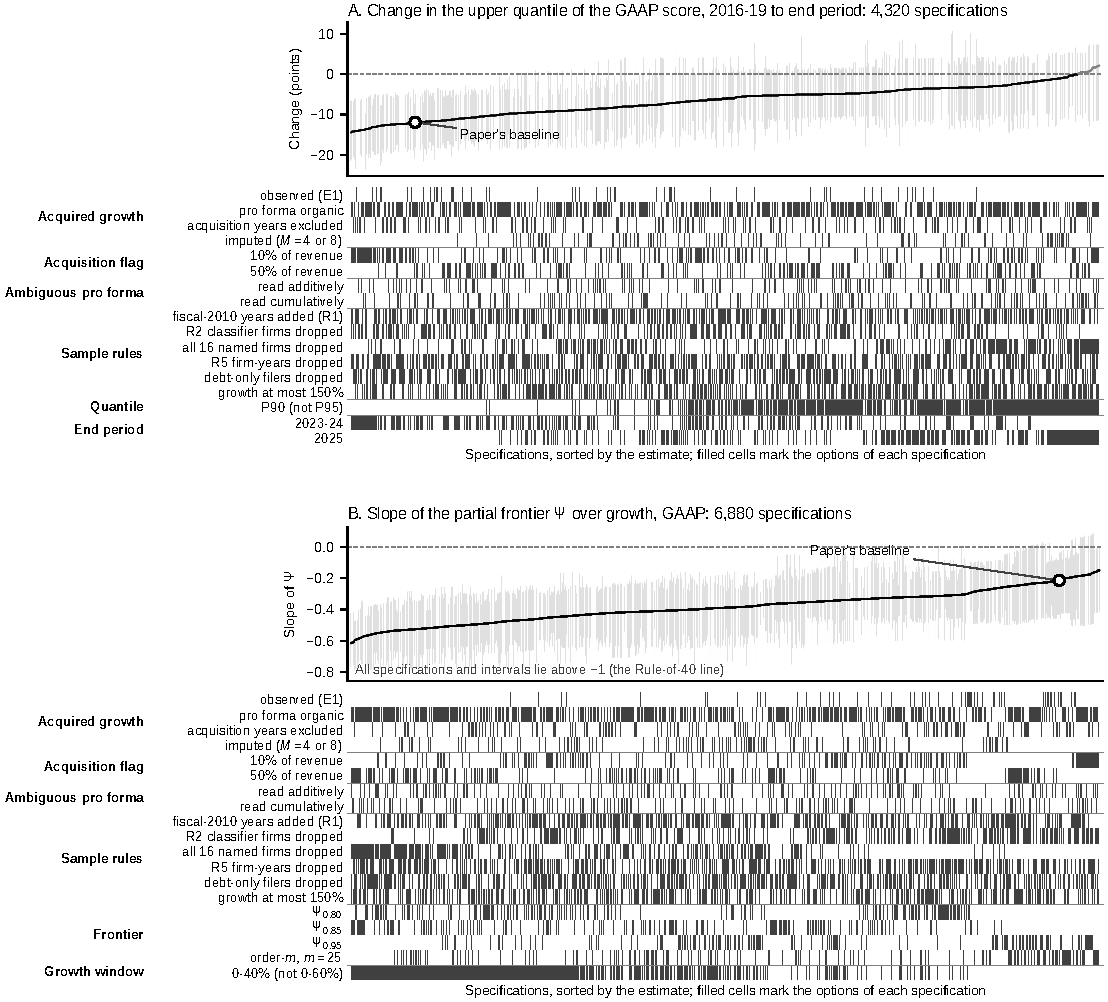
\includegraphics[width=\linewidth]{figures/fig_spec_curve.pdf}
\caption{Specification curves of two headline claims. A: change in the upper quantile of the GAAP score from 2016--19 to the end period, \ScTopOpN{} specifications sorted by the estimate; black, a decline; grey, a rise. B: slope of the partial frontier $\Psi$ over growth on the GAAP basis, \ScPsiOpN{} specifications with a defined slope. Open circles: the paper's baseline. Light vertical lines: 90\% firm-cluster percentile intervals of the specifications in the \ScBootK{} bootstrapped samples (\ScBootB{} replications). Below each curve, filled cells mark the options of each specification: every family of treatment of acquired growth, and for the other choices the options other than the paper's, so that a specification with no filled cell in a group takes the paper's option there. Generated by \texttt{code/spec\_curve.py}}\label{fig:spec_curve}
\end{figure}
